\chapter{Subordination and Coordination} \label{ch:subord-coord}
\is{subordination|(}\is{coordination|(}

\epigraph{consider the bridge:\\
how it must both\\
submit to and command\\
the space it spans}{}

\section{Introduction}

Language allows us to express not just individual ideas but relationships between ideas. Two fundamental ways we do this are through subordination\is{subordination!definition} and coordination\is{coordination!definition}. Each serves a distinct purpose: subordination creates hierarchies of dependency, while coordination joins elements of equal status.

Consider these three ways of connecting the same basic ideas:

\ea \label{ex:intro}
    \ea[]{\textit{Kim left. Pat came.}\hfill[separate]}
    \ex[]{\textit{The fact {\ob}that Kim left{\cb} enabled Pat's arrival.}\hfill[subordinate]}
    \ex[]{\textit{Kim left and Pat came.}\hfill[coordinate]}
    \z
\z

In (\ref{ex:intro}a), we have two independent statements. In (b), \textit{that Kim left} is subordinate\is{subordination!clausal embedding} to the main clause~-- it functions as a complement in the subject. In (c), the two clauses are coordinated~-- they stand as equals, simply joined by \textit{and}\is{coordinator!and@\textit{and}}\is{coordination}\is{coordinate}.

This contrast between hierarchy and equality runs deep in grammar. When we subordinate one clause to another, we're creating a relationship of dependence~-- one clause serves as a complement or modifier of an element in the other. When we coordinate elements, we're asserting their equal status in the structure, even if they differ in other ways.

The tools we use for these different relationships~-- subordinators like \textit{that} and \textit{whether}\is{subordinator!\textit{that}}\is{subordinator!\textit{whether}}, and coordinators like \textit{and}, \textit{or}, and \textit{but}\is{coordinator!or@\textit{or}}\is{coordinator!but@\textit{but}}~-- are small in number but they allow us to build complex meanings from simple parts, to show how ideas relate to each other, and to guide our audience through long chains of reasoning. These items function as markers\is{marker} rather than heads.

In this chapter, we'll explore how these two systems work, both separately and together. We'll see how subordination allows us to embed one thought within another, creating layers of meaning. We'll examine how coordination lets us build complex ideas while maintaining structural simplicity. And we'll discover how these two systems complement each other, giving us the flexibility to express almost any relationship between ideas we can imagine.

\section{Subordination}\label{sec:subordination}
\is{subordination!matrix vs main}\is{clause!matrix}\is{clause!main}\is{clause!subordinate}

When we communicate, we often need to express complex relationships between ideas. Sometimes one idea depends on another, or one thought serves to modify or explain another. This is where subordination comes in. \textsc{Subordination} is the grammatical process by which we make one clause a dependent in another.

A clause containing a subordinate clause is called the \textsc{matrix clause}, while a clause without a matrix is called a \textsc{main clause.} A clause can be both main and matrix as the following example shows.

\ea \label{ex:sub-basic}
    \ea[]{\textit{Kim left early.}\hfill[\textsc{main}]}
    \ex[]{\textit{She thinks {\ob}that Kim left early{\cb}.}\hfill[\textsc{subordinate}]}
    \ex[]{\textit{She thinks that Kim left early.}\hfill[\textsc{main/matrix}]}
    \z
\z

(\ref{ex:sub-basic}a) is a simple main clause. In (b), that same clause, in square brackets, has become subordinate~-- it's now a dependent within its matrix clause (c), which is also the main clause.

This pattern can be extended. In (\ref{ex:sub-basic2}), (\ref{ex:sub-basic}b) has changed from a main clause to a subordinate clause, while remaining the matrix clause for \textit{that Kim left}. In other words, a clause can not only be both main and matrix, but also subordinate and matrix.

\ea[]{\textit{I heard {\ob}that she thinks {\ob}that Kim left early{\cb}{\cb}.}\hfill[\textsc{subordinate}]}\label{ex:sub-basic2}
\z

No clause can be main and subordinate at the same time though. \textsc{Matrix} and \textsc{subordinate} are relational terms expressing one clause's position with respect to another. \textsc{Main clause}, though, reflects a syntactic type whose structure isn't always followed in the different subordinate clause types.

\subsection{Types of subordinate clauses}
\is{subordination!types}\is{content clause|(}\is{comparative clause|(}\is{relative clause}

English has three major types of subordinate clauses:\footnote{\textit{CGEL} makes a distinction between finite and non-finite subordinate clauses, of which there are various types, but I won't be taking those up here.} content clauses, comparative clauses, and relative clauses. Let's look at each in turn:

\ea \label{ex:sub-types}
    \ea[]{\textit{I doubt \uline{that we ordered enough books}.}\hfill[\textsc{content}]}
    \ex[]{\textit{More books arrived than \uline{we had ordered}.}\hfill[\textsc{comparative}]}
    \ex[]{\textit{The books \uline{that we ordered} arrived.}\hfill[\textsc{relative}]}
    \z
\z

Content clauses are the default case~-- they lack the special syntactic properties of relatives and comparatives. Relative clauses are the focus of \href{ch:relatives}{the next chapter}, so we'll consider content clauses first and then comparatives.

\subsubsection{Content clauses}
\is{content clause!declarative}\is{content clause!interrogative}\is{subordinator|(}\is{marker}

Content clauses have two main flavours: declarative and interrogative, as in (\ref{ex:content-types}).\footnote{Exclamative content clauses are also treated in \textit{CGEL}, but they're quite rare.}

\ea \label{ex:content-types}
    \ea[]{\textit{She said \uline{that it was genuine}.}\hfill[\textsc{declarative}]}
    \ex[]{\textit{She asked \uline{whether it was genuine}.}\hfill[\textsc{basic interrogative}]}
    \ex[]{\textit{She asked \uline{what made it genuine}.}\hfill[\textsc{focused interrogative}]}
    \z
\z

The words \textit{that} and \textit{whether} in (\ref{ex:content-types}a \& b) are doing important work~-- they're marking their respective clauses as subordinate. This brings us to an important new but very small category: \textsc{subordinator} (Sdr). The main members of this category are \textit{that}\is{subordinator!\textit{that} (declarative)} and \textit{whether}\is{subordinator!\textit{whether}}, along with \textit{if} (meaning `whether', not the conditional \textit{if})\is{subordinator!\textit{if} (\textit{whether})}. Subordinators are special because, unlike other lexical categories, they don't project phrases\is{phrase!no ``subordinator phrase''}. While nouns have NPs and verbs have VPs, subordinators don't have SdrPs. Instead, they function purely as markers, signalling how their clause relates to the larger structure. The tree structure is shown in Figure \ref{fig:sub-tree-sub}. (The triangles mean there's some hidden structure. See Chapter \ref{sec:more trees}.)

\begin{figure}
    \centering
    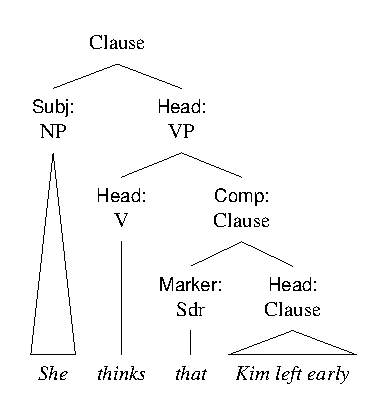
\includegraphics[width=0.55\linewidth]{figures/she thinks that kim left.pdf}
    \caption{Syntax tree showing subordination: \textit{that Kim left early} as a complement in \textit{She thinks that Kim left early}}\label{fig:sub-tree-sub}
\end{figure}
    

Notice how, in the subordinate structure, \textit{that} appears as a marker, not projecting its own phrase but simply signalling the start of the subordinate clause. A \textsc{marker} (Mk) is a kind of dependent that signals how its head relates grammatically to the larger structure.

Content clauses can function in various ways within the larger structure:

\ea \label{ex:content-funcs}
    \ea[]{\textit{I \uline{suspect} {\ob}that he left{\cb}.}\hfill[\textsc{in VP}]}
    \ex[]{\textit{The \uline{fact} {\ob}that he left{\cb} is clear.}\hfill[\textsc{in NP}]}
    \ex[]{\textit{I'm \uline{glad} {\ob}that he left{\cb}.}\hfill[\textsc{in AdjP}]}
    \ex[]{\textit{We can proceed \uline{provided} {\ob}that he left{\cb}.}\hfill[\textsc{in PP}]}
    \ex[]{\textit{\uline{Whether or not he left} is unclear.}\hfill[\textsc{subject}]}
    \ex[]{\textit{It's unclear \uline{whether or not he left}.}\hfill[\textsc{extraposed subject}]}
    \z
\z
\is{complement, complementation!in VP}\is{complement, complementation!in NP}\is{complement, complementation!in AdjP}\is{complement, complementation!in PP}\is{subject (Subj)!}\is{extraposition!subject}\is{complement, complementation!externalized}

\paragraph*{Declaratives} The marker (subordinator \textit{that}) in declarative content clauses can be obligatory, optional, or inadmissible, depending on the function of the clause:
\ea\label{ex:marker-need}
    \ea[]{\textit{\uline{That Kim left} surprised no one.}\hfill[obligatory]}
    \ex[]{\textit{I know \uline{{\op}that{\cp} Kim left}.}\hfill[optional]}
    \ex[]{\textit{We left before \uline{{\op}*that{\cp} Kim arrived}.}\hfill[inadmissible]}
\z\z
Subject clauses like (\ref{ex:marker-need}a) always need a marker. As complements, declaratives can mostly go with or without a marker, as in (b). The main exceptions to this are when they function as complements in PPs, as in (c).
\is{that-clause@\textit{that}-content clause}


\paragraph*{Interrogatives}\label{sec:sub-interrog}
\is{content clause!interrogative}\is{interrogative clause!subordinate vs main}\is{inversion!subject--auxiliary}\is{subject--auxiliary inversion}

Interrogative content clauses are interesting because they differ syntactically from main-clause interrogatives. While main-clause basic interrogatives can be identified by subject--auxiliary inversion (\textit{Did she accept?}), their subordinate counterparts mark their interrogative nature with \textit{whether} or \textit{if} instead:

\ea basic interrogatives\label{ex:int-sub}
    \ea[]{\textit{Did she accept?}\hfill[\textsc{main} inverted]}
    \ex[]{\textit{I wonder {\ob}whether she accepted{\cb}.}\hfill[\textsc{subordinate}]}
    \z
\z
\ea focused interrogatives
    \ea[]{\textit{How did we get here?}\hfill[\textsc{main} inverted]}
    \ex[]{\textit{I wonder {\ob}how we got here{\cb}.}\hfill[\textsc{subordinate}]}
    \z
\z

This is tough for learners of English. Beginners usually invert nothing, getting main-clause interrogatives wrong, while more experienced students, having figured out inversion, apply it everywhere, mis-structuring subordinate clause interrogatives. It's only at the much higher levels that students comfortably differentiate.

This structural difference between main and subordinate interrogative clauses is starting to break down though, as inversion continues its slow expansion\is{change in progress!inversion in subordinates}. Although it's still rare to see inverted interrogative content clauses in writing, examples like (\ref{ex:non-inverted-interrogative}) have become quite common in speech. In a few hundred years, inversion may be the norm for all interrogatives and the markers may become optional.

\ea[]{\textit{We need a story of {\ob}how did we get here{\cb}.}}\label{ex:non-inverted-interrogative}
\z

For now, though, a marker (usually \textit{whether} or \textit{if}) is always obligatory in basic interrogative content clauses. Otherwise, it would be impossible to distinguish them from unmarked declaratives in most cases.

\paragraph*{The mandative}
\is{mandative}\is{subjunctive}\is{modal auxiliary verb}\is{indicative}\is{varieties of English!AmE vs BrE (mandative)}

A special subtype of subordinate construction is the \textsc{mandative}, which occurs with predicates expressing requirement or necessity:

\ea \label{ex:mandative}
    \ea[]{\textit{It is essential {\ob}that he \uline{be} there{\cb}.}\hfill[\textsc{subjunctive}]}
    \ex[]{\textit{It is essential {\ob}that he \uline{should be} there{\cb}.}\hfill[\textsc{should}]}
    \ex[]{\textit{It is essential {\ob}that he \uline{is} there{\cb}.}\hfill[\textsc{indicative}]}
    \z
\z

The \textsc{subjunctive} variant uses the plain form of the verb, while the \textit{should} variant is (or at least used to be) more common in British English. American English tends to prefer the subjunctive. The \textsc{indicative} variant uses a regular tensed form.

This is a good example of how variations in subordinate clauses can carry subtle meaning differences and show regional preferences. For teaching purposes, it's worth noting that the indicative form is becoming more common, especially in informal contexts, though the subjunctive remains standard in formal writing.
\is{subordinator|)}

\subsection{Comparative clauses}
\is{comparative clause!definition}\is{comparison!inequality}\is{comparison!equality}\is{ellipsis!comparatives}

The second major type of finite subordinate clause is the comparative clause. These are clauses that complete a comparison, as in (\ref{ex:comparative-intro}).

\ea \label{ex:comparative-intro}
    \ea[]{\textit{The ice was thicker than {\ob}we expected{\cb}.}}
    \ex[]{\textit{She writes faster than {\ob}she speaks{\cb}.}}
    \ex[]{\textit{It doesn't cost as much as {\ob}I'd thought{\cb}.}}
    \z
\z

What distinguishes comparative clauses from content clauses is that they involve ellipsis~-- leaving out elements that can be recovered from context (see Section \ref{sec:ellipsis})\is{ellipsis!recoverability}. Look at (\ref{ex:comparative-ellipsis}), where the \dots indicate ellipsis.\footnote{In Section \ref{sec:subj-aux-inversion-and-fronting}, I introduced gaps. Gaps differ from ellipsis in that they're structural elements in trees; ellipsis is material semantically recoverable from context but not a syntactic element.}

\ea \label{ex:comparative-ellipsis}
    \ea[]{\textit{Kim read more books than {\ob}Pat read \dots{\cb}.}}
    \ex[]{\textit{Kim read more books than {\ob}Pat did \dots{\cb}.}}
    \ex[]{\textit{Kim read more books than {\ob}Pat{\cb}.}}
    \z
\z
\is{pro-form!\textit{do}/\textit{did} (VP pro-form)}

The first two variants show ellipsis, with (b) using the pro-form \textit{did} instead of repeating \textit{read}. The third (c) has \textit{Pat} as an NP complement, rather than a clausal complement. All three mean essentially the same thing.

Unlike in most cases of ellipsis, in comparative clauses, it's ungrammatical to supply the elided information (e.g., *\textit{Kim read more books than Pat read 20 books} or *\textit{It's not as deep as it is 20 cm wide}). The ellipsis is a key part of the clause type\is{comparative clause!obligatory ellipsis}. The structure of the comparative clause is shown in Figure \ref{fig:comp-tree}.

\begin{figure}
    \centering
    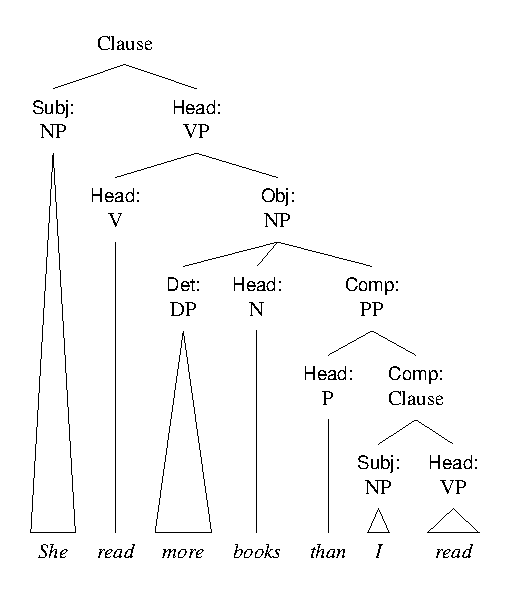
\includegraphics[width=0.7\linewidth]{figures/she read more books than I read.pdf}
    \caption{Syntax tree showing a comparative clause with ellipsis}\label{fig:comp-tree}
\end{figure}

Comparative clauses function as complements in a \textit{than} or \textit{as} PP, depending on the type of comparison that's being made.

\ea \label{ex:comp-markers}
    \ea[]{\textit{Kim is taller than {\ob}Pat is{\cb}.}\hfill[inequality]}
    \ex[]{\textit{Kim is as tall as {\ob}Pat is{\cb}.}\hfill[equality\footnote{The term \textit{equality} here may be somewhat misleading. The example means that Kim is \strong{at least} as tall as Pat, and may even be taller.}]}
    \z
\z
\is{preposition, preposition phrase (PP)!than@\textit{than}}\is{preposition, preposition phrase (PP)!as@\textit{as}}\is{adverb, adverb phrase (AdvP)!as@\textit{as} (degree)}

\textit{Than} in (\ref{ex:comp-markers}a) signifies inequality, while \textit{as} in (b) marks equality. The first \textit{as} is an adverb~-- we have the AdjP \textit{as tall}, with \textit{as} as a modifier~-- while the second is a preposition.

For English learners, comparative clauses pose several challenges:
\begin{itemize}[noitemsep]
    \item Understanding when and how much can be elided
    \item Mastering the different patterns for equality vs inequality
    \item Dealing with complex comparisons involving multiple elements
\end{itemize}

The good news is that comparative clauses follow fairly regular patterns, and learners can typically master the basic forms (\textit{taller than}, \textit{as tall as}) before tackling more complex structures.
\is{comparative clause|)}\is{content clause|)}

\section{Coordination}\label{sec:coordination}
\is{coordinator|(}\is{coordinate}\is{non-headed construction}\is{coordination|(}

While subordination creates relationships of dependency between clauses, \textsc{coordination} joins elements of equal syntactic status. At the heart of this system is a small closed class of words called \textsc{coordinators} (Crd), principally \textit{and}, \textit{or}, and \textit{but}. Like subordinators, coordinators function as markers.

Consider these examples:

\ea \label{ex:coord-basic}
    \ea[]{\textit{{\ob}Jane is a good teacher{\cb} {\ob}and her students really like her{\cb}.}}
    \ex[]{\textit{They offered us a choice of {\ob}red wine{\cb}, {\ob}white wine{\cb}, {\ob}or beer{\cb}.}}
    \ex[]{\textit{Her assistant is {\ob}very young{\cb} {\ob}but a quick learner{\cb}.}}
    \z
\z

The bracketed elements in these examples function as \textsc{coordinates}. This function can be realized by clauses as in (\ref{ex:coord-basic}a), NPs or other phrases as in (b), or, less commonly, a mixture of categories like the AdjP and NP in (c). The coordinators typically express distinct relationships: \textit{and} for addition, \textit{or} for alternatives, and \textit{but} for contrast.

What makes coordination different from the constructions we've seen before is that it's non-headed~-- no coordinate is the head of the whole construction. This non-headed nature is evident in a simple test: in most cases, you can replace the whole coordination with any one of its coordinates:

\ea \label{ex:coord-replace}
    \ea[]{\textit{Her assistant is very young.}}
    \ex[]{\textit{Her assistant is a quick learner.}}
    \z
\z

Both (\ref{ex:coord-replace}a) and (b) are grammatical alternatives to (\ref{ex:coord-basic}c). This is quite different from headed constructions like \textit{very young}, where you can use the head alone (\textit{she's young}) but not the dependent (\textit{*she's very}). The coordination structure is shown in Figure \ref{fig:coord-basic}.

\begin{figure}
    \centering
    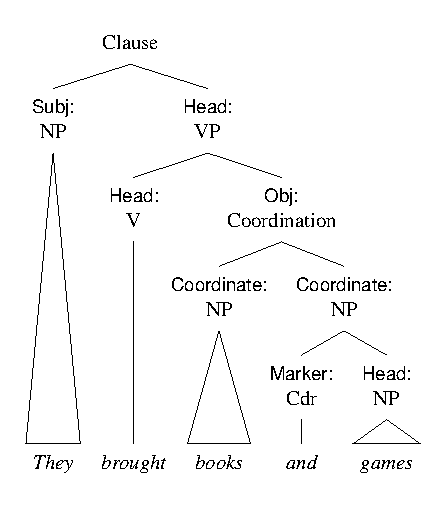
\includegraphics[width=0.65\linewidth]{figures/the brought books and games.pdf}
    \caption{Basic coordination with a marker: \textit{They brought books and games}}\label{fig:coord-basic}
\end{figure}

\subsection{Properties of coordination}
\is{coordination!multiple coordinates}\is{coordination!functional similarity}\is{fronting!ban with expanded coordinate}

Three key properties distinguish coordination from other constructions:

There's no grammatical limit on the number of coordinates (except with \textit{but}):
    
\ea \label{ex:coord-multiple}
    \textit{Nothing \uline{noble, sublime, profound, delicate, tasteful or even decent} can find a place.}
\z

The coordinates must be functionally similar~-- they need to be able to serve the same function when used alone:

\ea \label{ex:coordinate-function}
    \ea[]{\textit{I'll be back \uline{next week or at the end of the month}.}\hfill[time adjuncts]}
    \ex[*]{\textit{We're leaving \uline{Rome and next week}.}\hfill[object vs adjunct]}
    \z
\z

An expanded coordinate (one with its coordinator) can never be moved to the front:

\ea \label{ex:coord-front}
    \ea[]{\textit{They attended but they aren't members.}}
    \ex[*]{\textit{But they aren't members, they attended.}}
    \z
\z

\subsection{A note on sentence-initial coordinators}
\is{coordinator!sentence-initial}\is{discourse connector}\is{sentence-initial coordinator}

A prescriptive rule warns against beginning sentences with coordinators like \textit{and} or \textit{but}. This prohibition has no basis in English grammar or usage. Sentence-initial coordinators have been used by skilled writers throughout the history of English, including in this book~-- you'll find numerous examples in this and other chapters. While a sentence-initial coordinator can't join its sentence to the preceding one in a tight coordination (recall the fronting restriction in (\ref{ex:coord-front})), it can serve as a discourse connector, signaling how the new sentence relates to what came before. The only genuine constraint is a stylistic one: like any device, sentence-initial coordinators can become monotonous if overused. But used judiciously, they are a valuable tool for managing discourse flow and signaling text relationships.

\subsection{Types of coordination}
\is{coordination!symmetric}\is{coordination!asymmetric}\is{coordination!distributive}\is{coordination!joint}

The simplest distinction is between \textsc{symmetric} coordination, where the order of coordinates doesn't matter, and \textsc{asymmetric} coordination, where it does:

\ea \label{ex:coord-sym}
    \ea[]{\textit{I was hungry and tired.}\hfill[symmetric]}
    \ex[]{\textit{I got up and had breakfast.}\hfill[asymmetric]}
    \z
\z

In (\ref{ex:coord-sym}a), reversing the coordinates doesn't change the meaning. But in (b), the order implies sequence~-- getting up happened before breakfast.

We also distinguish between \textsc{distributive} and \textsc{joint} coordination:

\ea \label{ex:coord-dist}
    \ea[]{\textit{Kim and Pat are fine players.}\hfill[distributive]}
    \ex[]{\textit{Kim and Pat are a good pair.}\hfill[joint]}
    \z
\z

In (\ref{ex:coord-dist}a), the property of being a fine player applies to Kim and Pat individually. But in (b), being a good pair can only apply to them together~-- neither alone could be a pair.

\subsection{Marking coordination}
\is{coordination!asyndetic}\is{coordination!syndetic}\is{coordination!repeated coordinators}\is{correlative pair}

Coordination can be marked in several ways:
\begin{itemize}[noitemsep]
    \item With a coordinator: \textit{red and blue}
    \item Without any marker: \textit{red, white, blue}
    \item With repeated coordinators: \textit{red or white or blue}
    \item With correlative markers: \textit{both red and blue}
\end{itemize}

While coordinators typically express addition (\textit{and}), alternatives (\textit{or}), and contrast (\textit{but}), they can carry additional meanings in asymmetric coordination:

\ea \label{ex:coord-meaning}
    \ea[]{\textit{Pay within a week and you'll get a discount.}\hfill[conditional]}
    \ex[]{\textit{Pay within a week or you'll lose the discount.}\hfill[negative conditional]}
    \z
\z
\is{coordination!conditional reading}\is{coordination!negative conditional}

With the introduction of coordinators, we have now encountered all the major lexical categories in English except for interjections, as well as the main syntactic functions they serve in clauses.

\subsection{The structure of coordination}
\is{coordination!functional identity}\is{complement, complementation!coordination}\is{modification, modifier!coordination}

When we coordinate elements, they must share the same syntactic function. This means that while you can coordinate complements with complements or modifiers with modifiers, you can't coordinate a complement with a modifier. Compare:

\ea \label{ex:coord-function}
    \ea[]{\textit{We listened {\ob}to the teacher{\cb} {\ob} and the students{\cb}.}\hfill[complements]}
    \ex[]{\textit{We listened {\ob}Monday{\cb} and {\ob}Tuesday{\cb}.}\hfill[modifiers]}
    \ex[*]{\textit{We listened {\ob}to the teachers{\cb} and {\ob}Monday{\cb}.}\hfill[mixed functions]}
    \z
\z

The elements being coordinated (called \textsc{coordinates}) can come from any major phrase type~-- nouns, verbs, adjectives, prepositions, or larger phrases and clauses. What matters is that they're functioning in the same way in the larger structure.

\subsection{Coordination with and without markers}
\is{asyndeton}\is{serial comma}\is{coordination!correlative}

Coordination can occur with or without an explicit coordinator. When there's no coordinator, we call it \textsc{asyndetic} coordination:

\ea \label{ex:coord-marking}
    \ea[]{\textit{She brought {\ob}games{\cb}, {\ob}stories{\cb}, {\ob}songs{\cb}.}\hfill[asyndetic]}
    \ex[]{\textit{She brought {\ob}games{\cb}, {\ob}stories{\cb}, and {\ob}songs{\cb}.}\hfill[syndetic]}
    \z
\z

In addition to simple coordination with a single coordinator, we can have \textsc{correlative} coordination, where markers appear with multiple coordinates:

\ea \label{ex:coord-correlative}
    \ea[]{\textit{{\ob}Both{\cb} tired {\ob}and{\cb} hungry}}
    \ex[]{\textit{{\ob}Either{\cb} now {\ob}or{\cb} never}}
    \ex[]{\textit{{\ob}Neither{\cb} simple {\ob}nor{\cb} easy}}
    \z
\z

\subsection{Layered coordination}
\is{coordination!layered}

Sometimes coordinates themselves contain coordination, creating what we call layered coordination. Consider this example:

\ea \label{ex:coord-layered}
\textit{The story was {\ob}short and sweet{\cb} but {\ob}complex and thought-provoking{\cb}.}
\z

Here we have two main coordinates joined by \textit{but}, but each of these coordinates contains its own internal coordination with \textit{and}. This layering allows us to express complex relationships between ideas while maintaining clear structure. The layered structure is shown in Figure \ref{fig:coord-layered}.

\begin{figure}
    \centering
    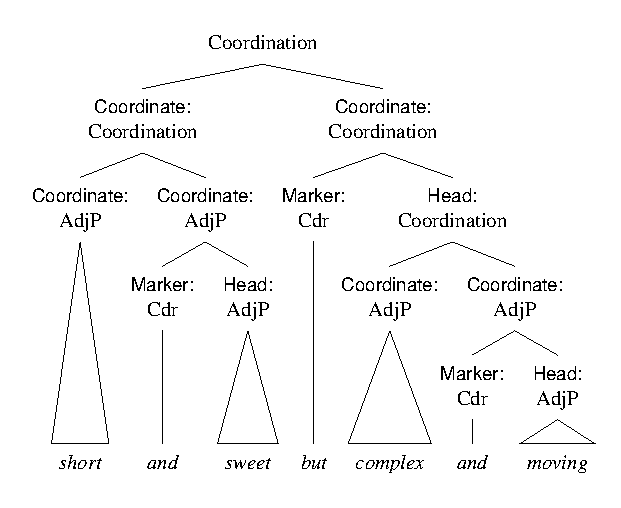
\includegraphics[width=0.9\linewidth]{figures/short and sweet but complex and moving.pdf}
    \caption{Layered coordination: \textit{short and sweet but complex and moving}}\label{fig:coord-layered}
\end{figure}


\subsection{Special types of coordination}
\is{coordination!comparative interface}

A particularly interesting type of coordination occurs in comparative structures:

\ea \label{ex:coord-comp}
    \ea[]{\textit{He's as tall as {\ob}or taller than{\cb} his brother.}}
    \ex[]{\textit{She writes more {\ob}but understands less{\cb} than before.}}
    \z
\z

These structures often involve complex relationships between the coordinates and their shared elements. Their interpretation requires understanding both the coordination and the comparative relationship.

\is{coordinator|)}\is{subordination|)}\is{coordination|)}

\section{Summary}

We've seen how English uses two fundamental systems to connect ideas: subordination and coordination. Though different in their mechanisms, both serve essential roles in building complex meanings from simpler parts.

Subordination, with its small set of markers like \textit{that} and \textit{whether}, allows us to embed one clause within another. This creates hierarchical relationships where one clause serves as part of another~-- as a complement in a VP (\textit{I know that she left}), an NP (\textit{the fact that she left}), an AdjP (\textit{glad that she left}), a PP (\textit{as good as it gets}), etc. In the next chapter, we'll focus on relative clauses, which typically function as modifiers in NPs.

Coordination, using the markers \textit{and}, \textit{or}, and \textit{but}, joins elements of equal status. Its apparent simplicity~-- just putting things together~-- belies its expressive power. Through coordination we can express addition (\textit{cats and dogs}), alternatives (\textit{now or never}), contrasts (\textit{difficult but rewarding}), and even relationships of time (\textit{she woke up and made coffee}) and condition (\textit{say that again and I'll leave}).

Together, these systems give English remarkable flexibility. We can layer coordinations within subordinate clauses (\textit{I heard that Kim and Pat left}), subordinate clauses within coordinates (\textit{Kim left and I think that Pat followed}), and build ever more complex structures. The result is a robust system for expressing how ideas relate to each other, all built from a small set of grammatical tools.
